\section{\textit{Statistical Learning}}

Per poter analizzare un \textit{learning algorithm} c'è bisogno di definire un 
modello matematico di come gli esempi $(x,y)$ siano generati. Nel contesto della
\textit{statistical learning} si assumerà che ogni esempio sia ottenuto attraverso
un'estrazione indipendente da una distribuzione di probabilità fissata su
$\X \times \Y$. Si scriverà $(X,Y)$ per sottolineare come 
\textbf{le due componenti di un esempio siano due variabili aleatorie}.

Assumere che ogni esempio $(x,y)$ sia la realizzazione di un'estrazione casuale 
\textbf{indipendente} da un'unica distribuzione $\D$, implica che ogni 
\textit{dataset} (come \textit{test} e \textit{training set}) sia un campione
statistico. L'indipendenza dei dati è in realtà violata in alcuni domini pratici.
Nonostante ciò, l'assunzione di indipendenza nei dati è estremamente utile dal
punto di vista della tracciabilità analitica del problema e funziona
sorpendentemente bene nella pratica.

\subsection{Definizioni}
Nel contesto della \textit{statistical learning} un problema è specificato da una
coppia $(\D,\ell)$, dove $\D$ è la distribuzione e $\ell$ la \textit{loss function}.

\subsubsection{Rischio statistico \texorpdfstring{$\ell_{\D}$}{lD}}
Le prestazioni di un predittore $h:\X \rightarrow \Y$ rispetto a $(\D,\ell)$ è 
valutata dal \textbf{rischio statistico}:
$$ \ell_{\D}(h) = \E[\ell(Y,h(X))] $$
che indica il valore atteso della \textit{loss function} su un esempio casuale 
$(X,Y)$ estratto da $\D$.

\subsubsection{Predittore ottimo di Bayes \texorpdfstring{$f^*$}{f*}}
Data $\D$, il miglior predittore possibile $f^*:\X \rightarrow \Y$ è detto 
\textbf{predittore ottimo di Bayes}:
$$ f^*(x) = \argmin_{\hat{y} \in \Y} \E[\ell(Y,\hat{y})\ | \ X=x] $$

\subsubsection{Rischio condizionato}
L'argomento di $\argmin$ di $f^*$, ovvero $\E[\ell(Y,\hat{y})\ | \ X=x]$, è detto
\textbf{rischio condizionato}. Il \textit{Bayes optimal predictor} quindi, è la 
predizione che minimizza il rischio condizionato. Un altro modo per scrivere il
rischio condizionato di un predittore $f$ è:
$$ \E[\ell(Y,\hat{y})\ | \ X=x] = \E[\ell(Y,f(X))\ | \ X=x] $$

\subsubsection{Rischio di Bayes \texorpdfstring{$\ell_{\D}(f^*)$}{lDF*}}
Essendo $f^*$ il miglior predittore possibile per $\D$ è ragionevole pensare che
esso abbia il rischio statistico migliore, ed è così; si ha infatti che il rischio 
$\ell_{\D}(f^*)$, detto \textbf{rischio di Bayes}, è il minore tra tutti i
predittori:
$$ \forall h \in \F \quad \ell_{\D}(f^*) \leq \ell_{\D}(h) $$
Tipicamente il rischio di Bayes è maggiore di zero vista la casualità delle
etichette.

\subsection{
    \texorpdfstring{$f^*$}{f*} e \texorpdfstring{$\ell_\D$}{lD*} nelle varie
    \textit{loss function}
}
Si valuteranno ora i predittori ottimi di Bayes per le varie \textit{loss function}.
\subsubsection{\textit{Quadratic loss}}

Sia $\ell(y,\hat{y}) = (y-\hat{y})^2 \ \text{con } \Y = \RN $.

Si analizzi il predittore ottimo di Bayes:
\begin{align}
    f^*(x) &= \argmin_{\hat{y}\in\RN} \E[(Y-\hat{y})^2 \ | \ X=x]  \notag\\
           &= \argmin_{\hat{y}\in\RN} \E[Y^2+\hat{y}^2-2\hat{y}Y\ | \ X=x]\notag\\[.6em]
        \multispan2{Per le varie proprietà del valore atteso si ha:\hfil} \notag\\[.6em]
           &= \argmin_{\hat{y}\in\RN}
            \left({\E[Y^2\ | \ X=x]}+\E[\hat{y}^2\ | \ X=x]-\E[2\hat{y}Y\ | \ X=x]\right)
            \notag\\[.6em]
           &= \argmin_{\hat{y}\in\RN}
           \left({\color{red}\E[Y^2\ | \ X=x]}+\E[\hat{y}^2\ | \ X=x]-2\hat{y}\E[Y\ | \ X=x]\right)
           \notag\\[.6em]
        \multispan2{Siccome $\argmin$ varia su $\hat{y}$, tutti {\color{red}i fattori che non ne dipendono}\hfil
        } \notag\\
        \multispan2{non incidono sul risultato; possono quindi essere tolti:\hfil
        } \notag\\[.6em]
        &= \argmin_{\hat{y}\in\RN}
           \left(\E[{\color{blue}\hat{y}}^2\ | \ X=x]-2\hat{y}\E[Y\ | \ X=x]\right)
           \notag\\[.6em]
        \multispan2{Non essendo ${\color{blue}\hat{y}}$ una variabile aleatoria:\hfil
           } \notag\\[.6em]
        &= \argmin_{\hat{y}\in\RN}
            \left({\color{blue}\hat{y}^2}-2\hat{y}\E[Y\ | \ X=x]\right) \notag
\end{align}
L'argomento di $\argmin$ è una funzione del tipo:
\begin{equation}
    F(\hat{y}) = \hat{y}^2 -2\hat{y}q \tag*{$q=\E[Y\ | \ X=x]$}
\end{equation}
Obiettivo di argmin è trovare il valore di $\hat{y}$ che minimizza $F$. Facendo 
un semplice studio di funzione si può trovare che $F$ è minimizzata quando:
$$
\begin{aligned}
    \multispan2{$F'(\hat{y}) = 2\hat{y}-2q$} \\
    \multispan2{Cerco il minimo:\hfill}\\
    F'(\hat{y}) &= 0\\
    2\hat{y}-2q &= 0\\
    \hat{y}     &=q\\
\end{aligned} \qquad \Rightarrow \qquad \hat{y}=\E[Y\ | \ X=x]
$$

\textbf{Si può quindi dire che}:
$$ f^*(x) = \E[Y\ | \ X=x]  = \E[Y\ | \ X]$$

Sostituendo il risultato appena mostrato nella formula del rischio condizionato
si ha:
$$ \begin{aligned}
    \ & \E[\ell(Y,\hat{y})\ | \ X=x] \\ 
    = \ &\E[(Y-f^*(X))^2\ | \ X=x] \\
    = \ &\E[(Y-\E[Y \ | \ X ])^2\ | \ X=x] \\
    = \ & \var[Y \ | \ X]
\end{aligned} $$

\textbf{Il rischio di Bayes sarà quindi}:
$$ \ell_\D(f^*) = \E[\var[Y \ | \ X]] \neq \var[Y] $$

Da notare che il valore atteso della varianza dato $X$ sia diverso dalla varianza;
per la legge della varianza totale si ha infatti che:
$$ \var[Y]-\E[\var[Y \ | \ X]] = \var[\E[Y \ | \ X]] $$

\subsubsection{\textit{Zero-one loss}}
Si guarderà ora la classificazione binaria dove $\Y = \{-1,1\}$.

Si definiscano due funzioni:
\begin{align}
\eta(x) = \Prob(Y=1 \ | \ X=x) \tag{\Prob \ è la funzione di probabilità}\\
\I\{A\} = \begin{cases}
1 & \text{si verifica $A$} \\
0 & \text{altrimenti}\\
\end{cases}\tag{$A$ è un evento}
\end{align}

La funziona \textit{zero-one loss} si potrà ora definire:
$$ \ell(y,\hat{y}) = \I\{\hat{y}\neq y\} $$
\textbf{Si analizzi il rischio statistico}:
$$
\begin{aligned}
    \ell_\D(h) &= \E[\ell(Y,h(X))]\\
               &= \E[\I\{h(X)\neq Y\}]\\
               &= \Prob(h(X)\neq Y)\\
\end{aligned}
$$
Di conseguenza \textbf{il predittore ottimo di Bayes è}:
\begin{align}
    f^*(x) &= \argmin_{\hat{y}\in\{-1,1\}} \E[(Y-\hat{y})^2 \ | \ X=x]  \notag\\
    &= \argmin_{\hat{y}\in\{-1,1\}} \E[
        \I\{Y=1\}\I\{\hat{y}=-1\}+\I\{Y=-1\}\I\{\hat{y}=1 \} \ | \ X=x
        ]  \notag\\[.6em]
        \multispan2{Si applichi la definizione di valore atteso:\hfill}\notag\\[.6em]
    &= \argmin_{\hat{y}\in\{-1,1\}} \Bigl(
        {\color{red}\Prob(Y=1 \ | \ X=x)}\I\{\hat{y}=-1\}+{\color{blue}\Prob(Y=-1 \ | \ X=x)}\I\{\hat{y}=1\}
    \Bigl)\notag\\
    &= \argmin_{\hat{y}\in\{-1,1\}} \Bigl(
        {\color{red}\eta(x)}\I\{\hat{y}=-1\}+{\color{blue}(1-\eta(x))}\I\{\hat{y}=1\}
    \Bigl)\notag\\
    &= \begin{cases}
        -1 & \eta(x)<1/2\\ 
        +1 & \eta(x)\geq1/2\\
    \end{cases}\notag
\end{align}
$f^*(x)$ predirrà quindi l'etichetta con la maggior probabilità quando condizionata
dall'istanza.

Infine è facile verificare che \textbf{il rischio di Bayes è}:
$$ \ell_\D(f^*)=\E[\min\{\eta(X),1-\eta(X)\}] $$

\subsection{Limitare il rischio}
Si vedrà ora come limitare il rischio statistico di un predittore.

\subsubsection{Stima del rischio}
Dato un predittore $h$ \textbf{non si può calcolare direttamente il suo rischio 
statistico $\ell_\D(h)$}; il motivo è semplice: \textbf{non si conosce $\D$} (se 
si conoscesse si potrebbe calcolare direttamente il predittore ottimo di Bayes).

Si dovrà quindi procedere ad ottenere una stima del rischio di un predittore $h$.
Per farlo 
\textbf{si userà il \textit{test set} $S'=\{(x_1',y_1'),\dots,(x_n',y_n')\}$};
in particolare si assumerà che $S'$ sia stato generato attraverso estrazioni 
indipendenti da $\D$ e che quindi:
\begin{equation}
    \quad (X_t',Y_t') \sim \D \tag*{$t=1,\dots,n$}
\end{equation}
Questo permette di affermare che:
$$ \E[\ell(Y',h(X'))] = \ell_{\D}(h) $$
Infine, usando come stimatore la media campionaria del rischio, \textbf{si può
avere una stima del rischio} attraverso il \textit{test set}, \textbf{ottenendo
di fatto il \textit{test error}}:
$$ \ell_{S'}(h) = \frac{1}{n}\sum_{t=1}^n \ell(y_t',h(x_t')) $$
È importante sottolineare che \textbf{la stima ha senso solo se $h$ non dipende
in alcun modo dal \textit{test set}}.

\subsubsection{Chernoff-Hoeffding}
Per poter calcolare quanto \quotes{buona} è la stima del rischio si può usare
il seguente risultato della legge dei grandi numeri.

\begin{lemma}[Chernoff-Hoeffding]\label{lem:chern-hoeff}
    Siano $Z_1,\dots,Z_n$ delle variabili aleatorie indipendenti e
    identicamente distribuite; sia $\mu$ il valore atteso e sia $0\leq Z_t\leq1$
    per ogni $t=1,\dots,n$. Allora per ogni $\varepsilon>0$ si ha che:
    $$ \Prob \left(
        \frac{1}{n}\sum_{t=1}^n Z_t > \mu + \varepsilon
    \right) \leq e^{\displaystyle-2\varepsilon^2n}
    \qquad \text{e} \qquad
    \Prob \left(
        \frac{1}{n}\sum_{t=1}^n Z_t < \mu - \varepsilon
    \right) \leq e^{\displaystyle-2\varepsilon^2n} $$
\end{lemma}
\vspace{1em}

Applicando il precedente lemma con $Z_t = \ell(Y_t',h(X_t')) \in [0,1]$ si
può trovare un intervallo di confidenza del rischio statistico:
$$\begin{aligned}
    \Prob \Bigl( |\ell_{S'}(h) - \ell_\D(h)| > \varepsilon \Bigl) &= 
        \Prob\Bigl((\ell_{S'}(h) > \ell_\D(h)+\varepsilon) \ \cup \ 
        (\ell_{S'}(h) < \ell_\D(h)-\varepsilon) \Bigl)\\
    &= \underbrace{\Prob\Bigl(\ell_{S'}(h) > \ell_\D(h)+\varepsilon\Bigl)}
        _{\leq \ e^{-2\varepsilon^2n}} \ + \
       \underbrace{\Prob\Bigl(\ell_{S'}(h) < \ell_\D(h)-\varepsilon \Bigl)}
       _{\leq \ e^{-2\varepsilon^2n}}
\end{aligned}$$
$$ \Downarrow $$
\begin{equation} \Prob \Bigl( |\ell_{S'}(h) - \ell_\D(h)| > \varepsilon \Bigl) 
 \ \leq \ 2e^{\displaystyle-2\varepsilon^2n} \label{eq:stat_risk_test}\end{equation}

Questo mostra che \textbf{la probabilità che il \textit{test error} 
$\ell_{S'}(h)$ differisca dal rischio statistico $\ell_\D(h)$ per più di 
$\varepsilon$, diminuisce esponenzialmente con il crescere della dimensione $n$ 
del \textit{test set}}.

Andando più nello specifico, si prenda un valore $\delta\in (0,1)$, uguale a
$2e^{-2\varepsilon^2n}$, e si isoli la $\varepsilon$:
\begin{align}
    2e^{-2\varepsilon^2n} &= \delta\notag\\[.15cm]
    e^{2\varepsilon^2n} &= \frac{2}{\delta}\notag\\[.15cm]
    2\varepsilon^2n &= \ln{\frac{2}{\delta}}\notag\\[.15cm]
    \varepsilon^2 &= \frac{1}{2n}\ln{\frac{2}{\delta}}\notag\\[.15cm]
    \varepsilon &= \sqrt{\frac{1}{2n}\ln{\frac{2}{\delta}}}\notag
\end{align}

Applicando i risultati appena mostrati su (\ref{eq:stat_risk_test}) si ottiene
infine:
$$ \Prob\left(|\ell_\D(h)-\ell_{S'}(h)| \leq 
\sqrt{\frac{1}{2n}\ln{\frac{2}{\delta}}}\right) \geq
1-\delta $$

\subsection{Decomposizione \textit{bias-variance}}
Si consideri un problema di \textit{learning} $(\D,\ell)$ e un \textit{learning
algorithm} $A$. Si scriverà $A(S)$ per indicare il predittore generato da $A$
preso in input il \textit{training set} $S$.

Sia $\Hm = \{h_1,\dots,h_m\}$ l'insieme dei predittori generati da $A$ su 
\textit{training set} di dimensione $m$; un predittore $h$ appartiene a $\Hm$ se
e solo se esiste un \textit{training set} $S$ di dimensione $m$ tale che $A(S)=h$:
$$ h\in\Hm \ \Leftrightarrow \ \exists S : |S|=m \ \wedge \ A(S)=h $$

Sia $h^*$ il miglior predittore di $\Hm$, ovvero il predittore con il rischio minimo
(ricordando che potrebbero essere più di uno):
$$ h^* \in \argmin_{h\in\Hm} \ell_\D(h) $$

Fissato un \textit{training set} $S$ di dimensione $m$ si indichi
$ h_S = A(S) \in \Hm $. Di seguito verrà mostrata la decomposizione
\textit{bias-variance}:
\begin{align}
    \ell_\D(h_S) =& \phantom{+.} \ell_\D(h_S) - \ell_\D(h^*)
    \tag{{\color{red}errore di stima o di variazione}}\\ 
        & +\ell_\D(h^*) - \ell_\D(f^*)
            \tag{{\color{blue}errore di approssimazione o di bias}}\\
        & +\ell_\D(f^*) \tag{rischio di Bayes}
\end{align}
Dove $f^*$ è il predittore ottimo di Bayes.
\begin{figure}[h]
    \centering
    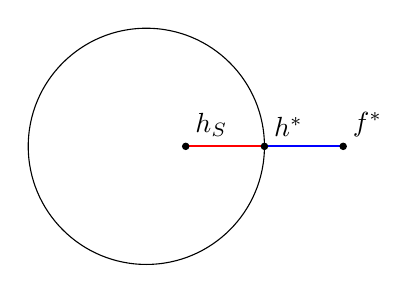
\begin{tikzpicture}[scale=.5]

    \draw (0,0) circle (3);
    
    \draw[thick,color=red](1,0) -- (3,0);
    \draw[thick,color=blue](3,0) -- (5,0);
    
    \draw[fill=black] (1,0) circle (.08);
    \node at (-2.75,2.75) {$\Hm$};
    \node[above right] at (1,0) {$h_S$};

    \draw[fill=black] (3,0) circle (.08);
    \node[above right] at (3,0) {$h^*$};

    \draw[fill=black] (5,0) circle (.08);
    \node[above right] at (5,0) {$f^*$};

\end{tikzpicture}
    \caption{Rappresentazione grafica della decomposizione \textit{bias-variance}}
\end{figure}

Si noti che:
\begin{itemize}
    \item Il rischio di Bayes non dipende da $A$;
    \item L'errore di approssimazione è grande quando $\Hm$ non contiene una buona
        approssimazione di $f^*$;
    \item L'errore di stima è grande quando $S$ non contiene abbastanza informazioni
        necessarie ad identificare $h^*$.
\end{itemize}

\subsection{\textit{Overfitting} e \textit{underfitting}}
Obiettivo di questo paragrafo è stabilire una connessione tra la decomposizione
\textit{bias-variance} e \textit{overfitting/underfitting}. Per farlo si prenda come
$A$ il \textit{learning algorithm} ERM su una classe di predittori arbritraria 
$\Hpred$  :
$$ A(S) = h_S = \argmin_{h \in \Hpred}\ell_S(h) $$
Si tenga poi conto del predittore ottimo $h^*$ di $\Hpred$:
$$ h^* \in \argmin_{h\in\Hpred} \ell_\D(h) $$
Si noti che $h_S$ è il miglior predittore che ERM riesce a trovare basando la stima
del rischio su $S$, mentre $h^*$ è il miglior predittore possibile esistente in
$\Hpred$, \textbf{che non dipende quindi da $S$}.

Il lemma \ref{lem:chern-hoeff} non può essere applicato direttamente in quanto 
$\ell_S(h_S)$ e $\ell_D(h_S)$ sono entrambi variabili aleatorie il cui valore atteso
non coincide necessariamente. Per poter quindi analizzare formalmente l'errore
di variazione di ERM si proceda come segue.

Per ogni \textit{training set} $S$ di dimensione $m$ si ha che:
\begin{align}
    \ell_D(h_S)-\ell_D(h^*) &= \phantom{|}\ell_D(h_S)-\ell_S(h_S)\phantom{|}
                +\phantom{|}\ell_S(h_S)-\ell_D(h^*) \notag\\[.6em]
                \multispan2{Per definizione $h_S$ minimizza il rischio stimato su $S$,
                si ha quindi\hfill}\notag\\
                \multispan2{che $\ell_S(h_S)\leq\ell_S(h^*)$:
                \hfill}\notag\\[.6em]
           &\leq\phantom{|}\ell_D(h_S)-\ell_S(h_S)\phantom{|}+\phantom{|}
                \ell_S(h^*)-\ell_D(h^*)\phantom{|} \notag\\
           &\leq |\ell_D(h_S)-\ell_S(h_S)|+|\ell_S(h^*)-\ell_D(h^*)| \notag\\
           &\leq 2\max_{h \in \Hpred} |\ell_S(h)-\ell_D(h)| \label{eq:var_err}
\end{align}
Concentrandosi ora sull'errore di variazione, si vuole capire quando, per ogni
$\varepsilon > 0$ si ha:
\begin{equation}
\ell_D(h_S)-\ell_D(h^*)>\varepsilon
\label{eq:var_err2}
\end{equation}
Unendo la disuguaglianza appena vista con (\ref{eq:var_err}) si ha:
$$
2\max_{h \in \Hpred} |\ell_S(h)-\ell_D(h)| \geq \ell_D(h_S)-\ell_D(h^*)
> \varepsilon
$$
Da cui:
\begin{align}
    2\max_{h \in \Hpred} |\ell_S(h)-\ell_D(h)| &> \varepsilon\notag\\
    \max_{h \in \Hpred} |\ell_S(h)-\ell_D(h)| &> \frac{\varepsilon}{2}\label{eq:var_err3}
\end{align}
$$ \Downarrow $$
\begin{equation}
    \exists h \in \Hpred : |\ell_S(h)-\ell_D(h)| > \frac{\varepsilon}{2}
    \label{eq:var_err4}
\end{equation}
Dai risultati (\ref{eq:var_err2}) e (\ref{eq:var_err4}) si evince che:
\begin{align}
    (\ref{eq:var_err2}) \quad &\Rightarrow \quad (\ref{eq:var_err4})\notag\\
    \ell_D(h_S)-\ell_D(h^*)>\varepsilon 
    \quad &\Rightarrow \quad \exists h \in \Hpred : |\ell_S(h)-\ell_D(h)|
    > \frac{\varepsilon}{2}\label{eq:var_err5}
\end{align}
La figura \ref{fig:prob_implication} mostra come:
\begin{equation}
    A \Rightarrow B \ \rightarrow \ \Prob(A) \leq \Prob(B) \label{eq:prob_impl}
\end{equation}
\begin{figure}[ht]
    \centering
    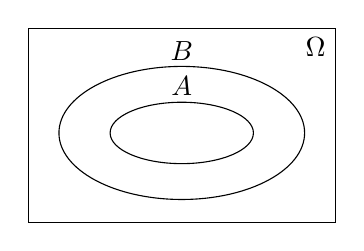
\begin{tikzpicture}[scale=1.3]

    \draw (0,0) rectangle (3,1.9);
    \node [below left] at (3,1.9) {$\Omega$};

    \begin{scope}[yshift=-3.5]
        \draw (1.5,1) ellipse (1.2 and .65);
        \draw (1.5,1) ellipse (.7 and .3);
        \node at (1.5,1.46) {$A$};
        \node at (1.5,1.8) {$B$};
    \end{scope}

\end{tikzpicture}
    \caption{\label{fig:prob_implication}}
\end{figure}

Da (\ref{eq:var_err5}) e (\ref{eq:prob_impl}) si ottiene che:
\begin{equation}
    \Prob(\ell_D(h_S)-\ell_D(h^*)>\varepsilon) \leq
    \Prob\left(\exists h \in \Hpred : |\ell_S(h)-\ell_D(h)|>\frac{\varepsilon}{2}
    \right) \label{eq:stat_risk_bound}
\end{equation}

\begin{figure}[ht]
    \centering
    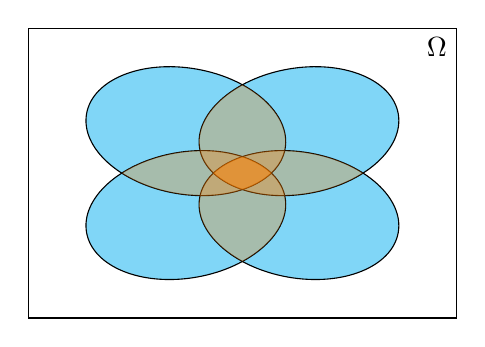
\begin{tikzpicture}[scale=1.6]

    \draw (-.2,-.2) rectangle (3.2,2.1);
    \node [below left] at (3.2,2.1) {$\Omega$};

    \def\circleOne{[
        rotate around={10:(1.5,0.95)},
        xshift=-.5cm,
        yshift=-.25cm,
    ] (1.5,0.95) ellipse (.8 and .5)};
    \def\circleTwo{[
        rotate around={10:(1.5,0.95)},
        xshift=.5cm,
        yshift=.25cm,
    ] (1.5,0.95) ellipse (.8 and .5)};
    \def\circleThree{[
        rotate around={-10:(1.5,0.95)},
        xshift=.5cm,
        yshift=-.25cm,
    ] (1.5,0.95) ellipse (.8 and .5)};
    \def\circleFour{[
        rotate around={-10:(1.5,0.95)},
        xshift=-.5cm,
        yshift=.25cm,
    ] (1.5,0.95) ellipse (.8 and .5)};

    \fill[cyan!50] \circleOne;
    \fill[cyan!50] \circleTwo;
    \fill[cyan!50] \circleThree;
    \fill[cyan!50] \circleFour;

    \draw \circleOne;
    \draw \circleTwo;
    \draw \circleThree;
    \draw \circleFour;

    \begin{scope}
        \clip \circleOne;
        \fill[orange,fill opacity=.3] \circleFour;
    \end{scope}
    \begin{scope}
        \clip \circleTwo;
        \fill[orange,fill opacity=.3] \circleThree;
    \end{scope}
    \begin{scope}
        \clip \circleOne;
        \fill[orange,fill opacity=.3] \circleThree;
    \end{scope}
    \begin{scope}
        \clip \circleTwo;
        \fill[orange,fill opacity=.3] \circleFour;
    \end{scope}

\end{tikzpicture}
    \caption{\label{fig:prob_union}}
\end{figure}

\textbf{Si guardi solo il caso in cui $\Hpred$ è finito ($|\Hpred|<\infty$)}.
\begin{align}
\Prob\left(\exists h \in \Hpred : |\ell_S(h)-\ell_D(h)|>\frac{\varepsilon}{2}\right)
&= \Prob\left(\bigcup_{h\in\Hpred} \left(|\ell_S(h)-\ell_D(h)|>
\frac{\varepsilon}{2}\right)\right)\notag\\
\multispan2{La probabilità dell'unione di più eventi non è uguale alla somma delle}\notag\\
\multispan2{probabilità dei singoli eventi in quanto alcuni eventi si potrebbero}\notag\\
\multispan2{sovrapporre come mostrato in figura \ref{fig:prob_union}. 
Tuttavia rappresenta un limite}\notag\\
\multispan2{superiore:\hfill}\notag\\
&\leq \sum_{h\in\Hpred}\Prob\left(|\ell_S(h)-\ell_D(h)|>\frac{\varepsilon}{2}\right)\notag\\
\multispan2{Si applichi il lemma \ref{lem:chern-hoeff}:\hfill}\notag\\
&\leq \sum_{h\in\Hpred}  2e^{\displaystyle-2\frac{\varepsilon^2}{4}m}\notag\\
&\leq \sum_{h\in\Hpred}  2e^{\displaystyle-\frac{\varepsilon^2m}{2}}\notag\\
&\leq |\Hpred|  2e^{\displaystyle-\frac{\varepsilon^2m}{2}}\label{eq:stat_risk_bound_2}
\end{align}
Da (\ref{eq:stat_risk_bound}) e (\ref{eq:stat_risk_bound_2}) si ha che:
\begin{equation}
\Prob(\ell_D(h_S)-\ell_D(h^*)>\varepsilon) \leq
|\Hpred|2e^{-m\varepsilon^2/2}
\label{eq:stat_risk_bound_3}
\end{equation}
Si chiami il lato destro $\delta$ e si isoli la $\varepsilon$:
\begin{align}
    2|\Hpred|e^{-m\varepsilon^2/2} &= \delta\label{eq:stat_risk_bound_4}\\[.15cm]
    e^{-m\varepsilon^2/2} &= \frac{\delta}{2|\Hpred|}\notag\\[.15cm]
    e^{m\varepsilon^2/2} &= \frac{2|\Hpred|}{\delta}\notag\\[.15cm]
    \frac{m\varepsilon^2}{2} &= \ln{\frac{2|\Hpred|}{\delta}}\notag\\[.15cm]
    \varepsilon^2 &= \frac{2}{m}\ln{\frac{2|\Hpred|}{\delta}}\notag\\[.15cm]
    \varepsilon &= \sqrt{\frac{2}{m}\ln{\frac{2|\Hpred|}{\delta}}}\label{eq:stat_risk_bound_5}
\end{align}
Concludendo, da (\ref{eq:stat_risk_bound_3}) si ha che:
\begin{align}
\Prob(\ell_D(h_S)\leq\ell_D(h^*)+\varepsilon) &\geq 1-|\Hpred|2e^{-m\varepsilon^2/2}\notag\\[.2cm]
\multispan2{Applicando (\ref{eq:stat_risk_bound_4}) e (\ref{eq:stat_risk_bound_5})
si ottiene:\hfill}\notag\\
\Prob\left(\ell_D(h_S)\leq\ell_D(h^*)+\sqrt{\frac{2}{m}\ln{\frac{2|\Hpred|}{\delta}}}\right) 
    &\geq 1-\delta\notag
\end{align}
Si ricordi che $m$ è la dimensione del \textit{training set}.

Fissato $m$, per poter diminuire lo scarto 
$\sqrt{\frac{2}{m}\ln{\frac{2|\Hpred|}{\delta}}}$ dell'errore di variazione di 
ERM, \textbf{bisogna diminuire $|\Hpred|$}. Diminuendo $|\Hpred|$ però si
incrementerebbe $\ell_D(h^*)$, il che farebbe aumentare l'errore di bias.

Alla luce di quest'analisi statistica, si può concludere che gli algoritmi ERM
generano predittori con un alto rischio (rispetto al rischio di Bayes) quando
c'è uno sbilanciamento tra l'errore di variazione e quello di bias.
In particolare:
\begin{itemize}
    \item Si verifica \textit{overfitting} quando l'errore di variazione domina
        l'errore di bias;
    \item Si verifica \textit{underfitting} quando l'errore di bias domina
        l'errore di variazione;
\end{itemize}